\documentclass[../TST.tex]{subfiles}
\begin{document}

\begin{pproblem}
A disc of radius $R$ and mass $m$ is placed on a horizontal surface. Initially the disc rotates with angular velocity $\omega$ about its axis of symmetry. The initial velocity of its centre of mass is $v$ (where $\omega R\gg v$). Find the initial friction force $F$ acting on the disc. The coefficient of friction between the disc and the surface is $k$. The acceleration due to gravity is $g$.
\end{pproblem}

\ifprob \else
	\begin{solution} We'll examine the friction on a piece of the disc at polar coordinates $(r,\,\theta)$, as shown. Its total velocity is a sum of the centre-of-mass velocity $\mathbf{v}$ and the rotational velocity $\boldsymbol{\omega}\times\mathbf{r}$. Given that $\mathbf{v}$ acts like a small correction to $\boldsymbol{\omega}\times\mathbf{r}$, the total velocity (and hence the friction force) will make some angle $\alpha$ with the $x$-axis that will equal $\theta$ plus some little adjustment $\beta$.
\begin{figure}[h]
	\begin{minipage}[b]{0.4\textwidth}
    \centering
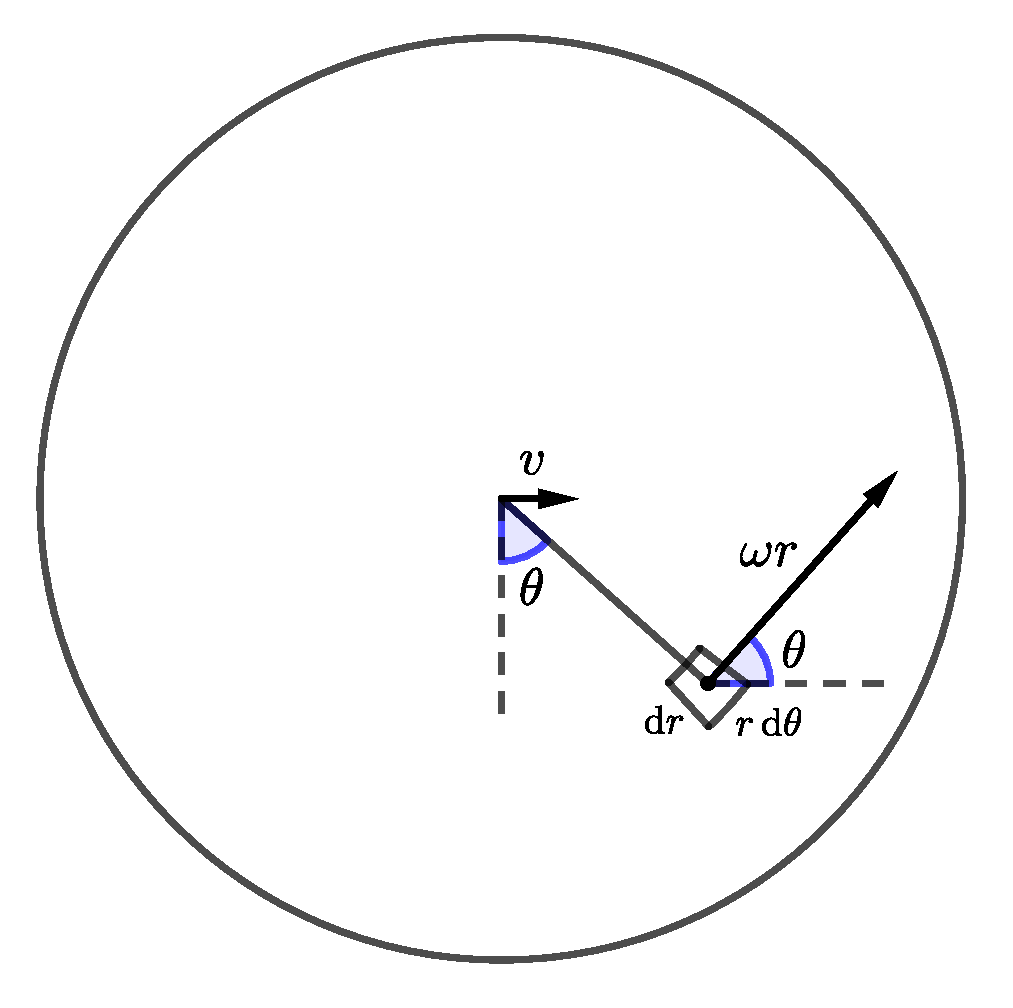
\includegraphics[width=\textwidth]{fig/a2016_s21.pdf}
	\end{minipage}\hfill
	\begin{minipage}[b]{0.5\textwidth}
		\centering
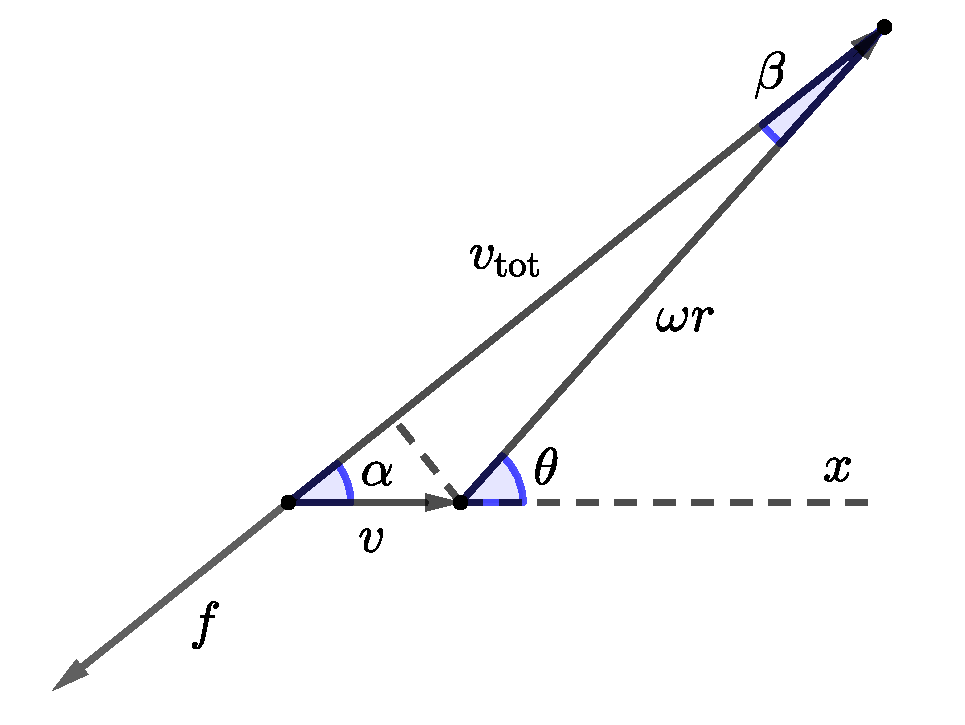
\includegraphics[width=\textwidth]{fig/a2016_s22.pdf}
	\end{minipage}
\end{figure}

We see that $\beta = \frac{v\sin{\theta}}{\omega r}\ll 1$ and $\alpha = \theta - \beta$. Then, it holds that
\begin{align*}
	\cos{\alpha}&=\cos{(\theta-\beta)}\approx \cos{\theta}+\beta\sin{\theta},\\
	\sin{\alpha}&=\sin{(\theta-\beta)}\approx \sin{\theta}-\beta\cos{\theta}
.
\end{align*}
The mass per unit area for the disc is $\sigma=\frac{m}{\pi R^2}$, from where the friction force on a small element can be expressed by $\mathrm{d}f=k\sigma (r \mathrm{d}r \mathrm{d}\theta)g$. The components of this force are
\begin{align*}
	\mathrm{d}f_x&=-k\sigma (r \mathrm{d}r \mathrm{d}\theta)g\cos{\alpha}=-k\sigma g (r \mathrm{d}r \mathrm{d}\theta)\left(\cos{\theta}+\frac{v}{\omega r}\sin^2{\theta}\right),\\
	\mathrm{d}f_y&=-k\sigma (r \mathrm{d}r \mathrm{d}\theta)g\sin{\alpha}=-k\sigma g (r \mathrm{d}r \mathrm{d}\theta)\left(\sin{\theta}-\frac{v}{\omega r}\sin{\theta}\cos{\theta}\right) .
\end{align*}
To get the total force, we integrate these from $0$ to $2\pi$ in $\theta$ and between $0$ and $R$ in $r$. The only angular term that doesn't integrate to zero is the $\sin^2{\theta}$ in $\mathrm{d}f_x$. It's well-known that the average value of $\sin^2{\theta}$ in any block of length $\pi$ is $\frac{1}{2}$, so the integral between  $0$ and $2\pi$ evaluates to $\frac{1}{2}\cdot 2\pi = \pi$. We reach
\begin{equation*}
	f=-\int_0^R k\sigma g \left(\frac{v}{\omega}\right) \pi \mathrm{d}r=\boxed{-kmg \left(\frac{v}{\omega R}\right).}
\end{equation*}
This is a small quantity and it reduces to zero when $v\rightarrow 0$, as expected.
\end{solution}
\fi
\end{document}
